\documentclass{llncs}
\usepackage{amssymb}
\usepackage{color}
\usepackage{pgf,pgfarrows,pgfnodes,pgfautomata,pgfheaps,pgfshade}
\usepackage{tikz}
\usetikzlibrary{arrows,decorations.pathmorphing,backgrounds,positioning,fit,petri}
\usepackage{amsmath}

\begin{document}

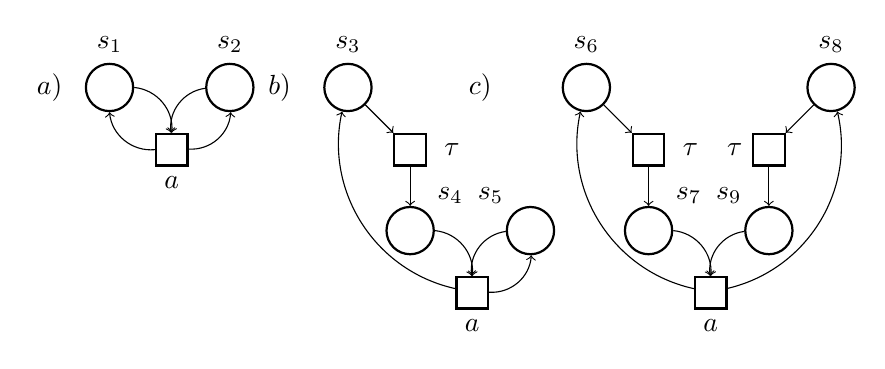
\begin{tikzpicture}[
every place/.style={draw,thick,inner sep=0pt,minimum size=6mm},
every transition/.style={draw,thick,inner sep=0pt,minimum size=4mm},
bend angle=45,
pre/.style={<-,shorten <=1pt,>=stealth,semithick},
post/.style={->,shorten >=1pt,>=stealth,semithick}
]
\def\eofigdist{2.4cm}
\def\eodist{0.5}
\def\eodisty{0.9}

\node (a) [label=left:$a)\quad $]{};

\node (q1) [place] [label={above:$s_1$} ] {};
\node (q2) [place] [right=\eodisty of q1,label={above:$s_2$}] {};
\node (f1)[transition][below right=\eodist of q1,label=below:$a$]{};

\draw  [->, bend left] (q1) to (f1);
\draw  [->, bend left] (f1) to (q1);
\draw  [->, bend right] (q2) to (f1);
\draw  [->, bend right] (f1) to (q2);

% seconda rete
  
 
\node (b) [right={2.5cm} of a,label=left:$b)\;\;$] {};

\node (p1) [place]  [right=\eofigdist of q1,label=above:$s_3$] {};
\node (s1) [transition] [below right=\eodist of p1,label=right:$\;\tau$] {};
\node (p2) [place] [below =\eodist of s1,label=above right:$s_4$]{};
\node (p3) [place] [right=\eodisty of p2,label=above left:$s_5$]{};
\node (s2) [transition] [below right=\eodist of p2,label=below:$a$] {};

\draw  [->] (p1) to (s1);
\draw  [->] (s1) to (p2);
\draw  [->, bend left] (p2) to (s2);
\draw  [->, bend left] (s2) to (p1);
\draw  [->, bend right] (p3) to (s2);
\draw  [->, bend right] (s2) to (p3);


% terza rete
  
 
\node (c) [right={2.3cm} of b,label=left:$c)\;\;$] {};

\node (v1) [place]  [right=\eofigdist of p1,label=above:$s_6$] {};
\node (t1) [transition] [below right=\eodist of v1,label=right:$\;\tau$] {};
\node (v2) [place] [below =\eodist of t1,label=above right:$s_7$]{};
\node (v3) [place] [right=\eodisty of v2,label=above left:$s_9$]{};
\node (t2) [transition] [below right=\eodist of v2,label=below:$a$] {};
\node (t3) [transition] [above=\eodist of v3,label=left:$\tau$] {};
\node (v4) [place] [above right=\eodist of t3,label=above:$s_8$]{};

\draw  [->] (v1) to (t1);
\draw  [->] (t1) to (v2);
\draw  [->, bend left] (v2) to (t2);
\draw  [->, bend left] (t2) to (v1);
\draw  [->, bend right] (v3) to (t2);
\draw  [->, bend right] (t2) to (v4);
\draw  [->] (v4) to (t3);
\draw  [->] (t3) to (v3);

 
\end{tikzpicture}

\end{document}